\section{Punto de Vista de Comportamiento de Aplicación}

\subsection{Modelo de comportamiento de Aplicación}
\begin{figure}[h!]
	\centering
	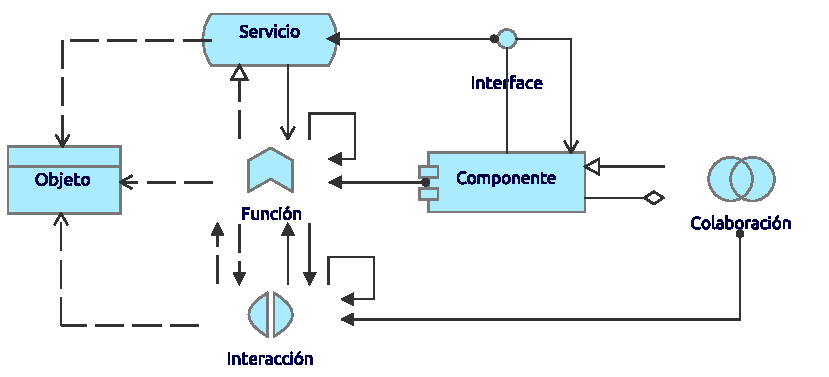
\includegraphics[width=.8\linewidth]{imgs/modelo/CmtoAplicacion}
	\caption{Modelo Comportamiento de Aplicación}
\end{figure}

El punto de vista del comportamiento de aplicaciones describe el comportamiento o el funcionamiento de los diferentes componen entes de la aplicación. Este punto vista busca trasmitir que finalidad tiene cada componente buscando mostrar una descripción breve de las actividades que realizan estos componentes.

\newpage

\subsection{Caso  de comportamiento de Aplicación}
\begin{figure}[h!]
	\centering
	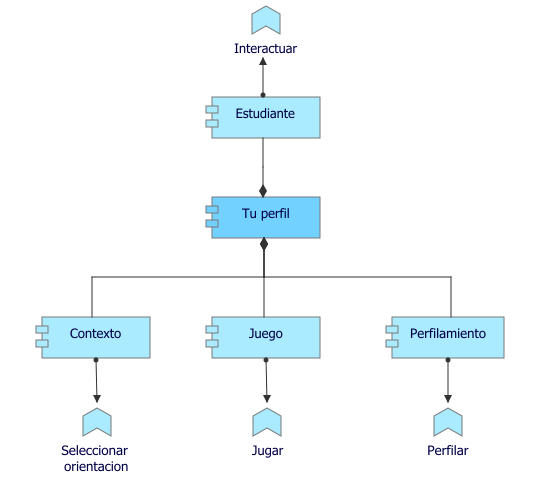
\includegraphics[width=.8\linewidth]{imgs/caso/aplicacion/comportamiento_aplicacion}
	\caption{Caso comportamiento de Aplicación}
\end{figure}

Para el caso de estudio nuestro orquestador es la aplicación Tu perfil el cual permite la comunicación entre los diferentes componentes. El componente estudiante realiza la interacción y comunicación por medio del orquestador (Tu perfil) hacia el juego y la obtención de su perfilamiento. El componente contexto es la base de datos que permite a el componente de perfilamiento realizar un análisis de los resultados obtenidos por el componente Juego, y así compararlos con el contexto proporcionando una orientación vocacional al estudiante.

\newpage